\let\textcircled=\pgftextcircled
\chapter{Problem Definition}
\label{chap:intro}

\initial{C}urrently, businesses globally have to communicate across multiple departments and management systems to facilitate cross-company transactions, leading to costly mistakes, opaque interaction histories, high administration costs and long delays for the transference of capital to be processed. Business blockchains, an innovative solution to this global issue, are reinventing how transactions are managed. They can take time and costs out of almost any process, enabling near real-time operations. And they deliver a high degree of accuracy and control, with much less risk than many alternatives. Due to the immutable nature of the blockchain, a transparent record of all transactions is kept which can be utilised for bookkeeping and taxation purposes while also preventing fraudulent behaviour as all transactions are recorded and can be reproduced for litigious reasons. The business blockchain that is being created, therefore, will help supply chain partners and corporations globally by creating a complete, transparent, tamperproof history and facilitation of the information flows, inventory flows, and financial flows in transactions. This permissioned blockchain will outperform current enterprise resource planning solutions as it is able to manage all transactions extremely quickly and efficiently, through sharing the load of computation across all nodes in the blockchain. An example of the differences between conventional record keeping and blockchain for a transaction is shown below. \\

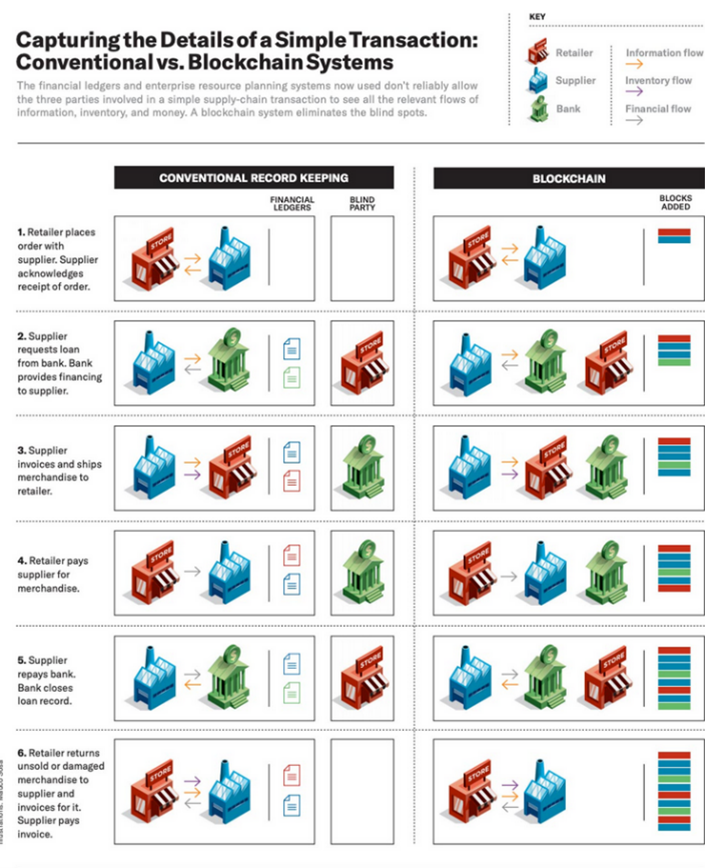
\includegraphics[width=\linewidth]{figures/vs.png} \\

The blockchain that is being developed is a proof of concept that will show the core functionality of permissioned blockchains and the benefits it produces. It will be compatible for all businesses as a node will be able to run on a server setup by the development team and users can interface with the system via a user-friendly web frontend to manage transactions and assets. The assets, labour and even items such as orders / invoices within each company will be tokenised on the blockchain so that businesses can interact with other businesses over the blockchain. Though it most commonly refers to the tokenization of financial or fungible assets, such as shares in a company or a quantity of gold, asset tokenization can hypothetically refer to the tokenization of any material or nonmaterial thing possessing monetary value: everything from a piece of art to a patent to an hour of a skilled worker’s time. This process of tokenization creates a bridge between real-world assets and their trading, storage and transfer in a digital world. Another example if the blockchain was to be used in Consultancy is we would enter the number of hours worked on the client for the month on the blockchain as a proposal for an invoice. When the client accepts the number of hours, the hours are posted to the blockchain, and the smart contract (explained in the following) executes the invoice creation based on the agreed hours and prices. \\

Although the functionality of transferring fungible and non-fungible assets will be implemented into the software solution, the legal processes surrounding the binding of assets will be implemented in the future. These legal proceedings are outside the scope of this project as they would require communication with governing institutions, intricate understanding of taxation law and connecting software solutions with the strenuous obligations of regulatory frameworks. \\

For the purpose of this conceptual design, I will utilise a main, “converge” token that is not truly backed by US Dollar or another asset, but in production, would be. The manner in which the tokens will be bound to physical assets is through the creation of a stable coin which reassures businesses will not have to consider the fluctuations of token value. To make this collateralised stable coin I would need to own the fiat or assets in which the token was based upon, as ‘collateral’ or conduct an exchange agreement with a bank in which the converge tokens could be converted into the local fiat currency. \\



